%%%%%%%%%%%%%%%%%%%%%%%%%%%%%%%%%%%%%%%%%%%%%%%%%%%%%%%%%%%%%%%%%%%%%%%%%%%%%%%%
%Objetivo: Propor um conjunto de recomendações de melhorias para as FGRM's
%Autores: Vagner Clementino <vagnercs@dcc.ufmg.br>
%		  Rodolfo Resende <rodolfo@dcc.ufmg.br>
%Criação: dom fev 26 12:49:27 BRT 2017
%Modificação: qui mar  9 20:54:30 BRT 2017
%Revisão:
%%%%%%%%%%%%%%%%%%%%%%%%%%%%%%%%%%%%%%%%%%%%%%%%%%%%%%%%%%%%%%%%%%%%%%%%%%%%%%%%
\chapter{Sugestões de Melhorias para as FGRM's}
\label{ch:sug_melhoria}

\section{Introdução}
\label{sec:sug_melhoria_intro}

Conforme já foi discutido nesta dissertação é inegável a importância das
Ferramentas de Gerenciamento de Requisições de Mudança \@-\@ FGRM no contexto da
manutenção de software. Conforme apresentado na
Seção~\ref{sec:caracterizacao_ferramentas} este tipo de sistema oferece suporte
ao relato das Requisições de Mudança \@-\@ RM, ao processo de atribuição das
RM's ao desenvolvedor mais apto, integração com Sistemas de Controle de Versão
\@-\@ SCV, dentre outras funcionalidades. Os usuários deste tipo de software, em
especial os ligados à manutenção de software, se mostraram, em geral,
satisfeitos com as funcionalidades oferecidas para o desempenho do seu trabalho.
O percentual de cerca de 90\% dos par\-ti\-ci\-pan\-tes da pesquisa descrita no
Capítulo~\ref{ch:pesquisa-profissionais} fizeram uma avaliação positiva, ao
mesmo tempo que a mesma quantidade de respondentes afirmam que recomendariam a
FGRM que utilizam para um novo projeto.

Não obstante, naquele mesmo levantamento, ao questionarmos se o profissional
sentiria falta de determinada funcionalidade, do qual listamos algumas, cerca de
15\% afirmaram não necessitar dos itens apontados em sua rotina de trabalho. A
partir desta última informação podemos inferir que os desenvolvedores estão
satisfeitos com a ferramenta utilizada, contudo, \textit{não conhecem ou não têm
	acesso ao potencial de funções que este tipo software pode oferecer}.

Diante do exposto, entendemos que podemos contribuir com o estado a\-tu\-al das
funcionalidades das FGRM's apresentando um conjunto de sugestões de melhorias.
As sugestões foram compiladas utilizando os resultados obtidos nesta
dissertação, especialmente com base nos
Capítulos~\ref{ch:mapeamento-sistematico} e~\ref{ch:pesquisa-profissionais}, na
Seção~\ref{sec:caracterizacao_ferramentas} e nos estudos que propõem melhorias
para as FGRM~\cite{zimmermann2009improving, bettenburg2008makes, singh2011bug}.
Estas recomendações podem ser utilizadas por pesquisadores interessados em
conduzir estudos sobre melhoria da produtividade dos desenvolvedores mediante o
uso das FGRM's. Além disso, os responsáveis pelo desenvolvimento deste tipo de
software podem utilizar este conjunto a fim de implementar futuras versões do
projeto. Na mesma linha, os profissionais envolvidos em manutenção de software
podem desenvolver extensões (plugins) para as FGRM com base no que foi proposto
de modo a utilizar as melhorias propostas neste estudo em sua rotina de
trabalho.

Este capítulo está organizado da seguinte forma: a
Seção~\ref{sec:sug_melhoria_melhorando_as_ferraementas} apresenta as sugestões
de melhoria do qual acreditamos poderia ser implantadas nas FGRM's, cada
sugestão apresenta foi seguida de uma breve justificativa de como foi obtida e
dos motivos de sua implementação; na
Seção~\ref{sec:sug_melhoria_avaliacao_das_melhorias} realizamos a avaliação das
sugestões que foram propostas, onde solicitamos a opinião de profissionais que
participam de projetos de código aberto que desenvolvem FGRM's; na
Seção~\ref{sec:sug_melhoria_discussao} discutimos os resultados obtidos do
processo de avaliação; na Seção~\ref{sec:sug_melhoria_ameacas} apresentamos as
ameaças à validade deste capítulo; encerramos esta parte do estudo com um breve
resumo na Seção~\ref{sec:sug_melhoria_resumo}.

\section{Sugestões de Melhorias para as FGRM's}
\label{sec:sug_melhoria_melhorando_as_ferraementas}

Nesta seção apresentamos um conjunto de recomendações de melhorias das
funcionalidades das FGRM's. As sugestões propostas não estão vinculadas
exclusivamente à melhorias de funcionalidades já existentes neste tipo de
ferramenta. O que está sendo proposto pode representar o desenvolvimento de um
novo tipo de comportamento para as FGRM's. Cabe-nos ressaltar que o conjunto
proposto não é exaustivo e é baseado nos resultados desta dissertação. Além
disso não houve compromisso com as dificuldades operacionais que implementação
das funcionalidades podem estar relacionadas, mesmo porquê avaliar esta
complexidade está fora do escopo deste estudo. É possível que algumas das
su\-ges\-tões propostas já estejam implementadas de maneira parcial ou integral
em alguma FGRM\@.  Contudo, não é possível validar esta premissa por conta de
volume de ferramentas disponíveis quando esta dissertação foi escrita.

Conforme discutido na
Subseção~\ref{subsec:man_visao_geral_papeis_na_manutencao_de_software} o
responsável por reportar uma RM pode ser tanto um usuário do sistema quando um
membro da equipe de desenvolvimento/manutenção. Neste caso existem diferentes
níveis de conhecimento sobre o sistema. Este diferente nivelamento pode
acarretar em diferentes níveis de qualidade do que é relato. Esta situação pode
causar atraso na análise da RM por falta da informação necessária a sua
resolução. Alguns estudos demonstram que, do ponto de vista dos desenvolvedores,
a falta de informação tais como etapas para reproduzir e registro de pilha de
ativação (stack tracke) dificultam mais o trabalho do que relato de problemas
(bugs) duplicados~\cite{bettenburg2008makes, bettenburg2007quality}. Neste
linha, estes estudos se dedicam a minimizar o problema através da análise da
qualidade do que é relatado em uma RM\@. A premissa é que o responsável pelo
relato deva ter ciência das informações que são necessárias à resolução do que
foi solicitado. Com este objetivo apresentamos a sugestão de desenvolvimento de
funcionalidade conforme descrito a seguir.

\sugestao{01}{As FGRM's devem fornecer um retorno (\textit{feedback}) da
	qualidade do relato realizado em uma RM.}

As RM's permitem a inclusão de código fonte em diversas etapas do seu ciclo de
vida. O código pode ser incluído durante a sua criação, nas discussões
realizadas para a sua resolução ou mesmo quando ela é concluída, onde recebe o
nome de \textit{patch.} Esta informação é bastante relevante para o projeto do
qual a RM faz parte, contudo, as FGRM's não permitem a sua recuperação, por esta
razão apresentamos a \textit{Sugestão 02}.

\sugestao{02}{As FGRM's devem possibilitar a busca por código fonte contido em
	seu relato, comentários ou anexos.}

Caso seja possível identificar que um \textit{Reportador} tem por hábito relatar
RM's que sejam relevantes ao projeto de software, tais requisições deveriam
receber algum tipo de etiqueta de modo a diferenciá-las dentro da FGRM\@.
Segundo o nosso entendimento uma RM pode ser classificada como relevante se
descreve um problema que afeta um grande número de usuários do sistema ou
representa uma falha de segurança do software. Além disso deve ser redigida de
forma clara e fornecer as informações necessárias para sua solução. O grau de
relevância de determinada RM pode variar em diferentes projetos e pode depender
de critérios subjetivos de quem analisa. Com objetivo de diferenciar as RM's
deste perfil de reportadores apresentamos a \textit{Sugestão 03}.

\sugestao{03}{As FGRM's devem diferenciar as RM'S criador por reportadores que
	historicamente relatam com qualidade e relevância.}

No ciclo de vida de uma RM, conforme discutido na
Subseção~\ref{subsec:man_visao_geral_papeis_na_manutencao_de_software}, após a
verificação de que a RM foi incorporada com sucesso ao software, ela é movida
para o estado \textit{Fechado (Closed)} e deixa de estar atribuída a determinado
desenvolvedor ou analista de qualidade. Caso um desenvolvedor queria acessá-la
novamente deverá utilizar o identificador da RM a fim de recuperá-la na FGRM\@.
Este histórico de trabalho do desenvolvedor pode ser útil na resolução de
eventuais RM que surjam posteriormente no projeto. No levantamento mediante
questionário, apresentado no Capítulo~\ref{ch:pesquisa-profissionais}, alguns
participantes relataram o desejo de uma funcionalidade  que gerencie este
histórico conforme apresentado a seguir. Por esta razão apresentamos a
\textit{Sugestão 04}.

\begin{itemize}
	\item Conforme relato dos participantes eles gostariam:
	\begin{itemize}
		\item \textit{``The ability to clearly visualize how many tickets are at
				the to do, in progress, to validate or done steps.''}.
		\item \textit{``History tracking, commenting, attachments, priority
				setting, task assignment, tie in with deployment systems.''}
	\end{itemize}
\end{itemize}

\sugestao{04}{As FGRM's devem permitir acesso facilitado para as $n$ últimas
	RM's que foram analisadas por um desenvolvedor.}

\section{Avaliação das Melhorias Propostas}
\label{sec:sug_melhoria_avaliacao_das_melhorias}

Este Capítulo se propôs apresentar um conjunto de sugestões que foram
construídas tomando como base a literatura da área e os resultados e
contribuições desta dissertação. Com o objetivo de avaliar a relevância e o grau
de facilidade de implementação das recomendações propostas, conduzimos um
levantamento mediante questionário com profissionais que contribuem em projeto
de código aberto hospedados no Github. A metodologia utilizada na condução do
levantamento é descrita na próxima subseção.

\subsection{Metodologia Levantamento com Questionário}
\label{sub:sug_melhoria_metodologia_levantamento}

Conforme discutido com maior detalhes no
Capítulo~\ref{ch:pesquisa-profissionais} um levantamento com questionário,
conhecido na literatura como \textit{Survey}, é uma abordagem de coleta e
análise de dados na qual os participantes respondem a perguntas ou declarações
que foram desenvolvidas antecipadamente~\cite{kasunic2005designing}. Para
realizarmos a coleta dos dados foi utilizado um questionário eletrônico. O
processo de seleção dos participantes, o desenho do questionário e como foi
realização a sua aplicação estão descritos na próximas subseções.

\subsubsection{Seleção dos Participantes}
\label{ssub:sug_melhoria_selecao_participantes}

Ficou definido que o público-alvo deste questionário seria profissionais que
estejam ligados ao processo de desenvolvimento e manutenção de FGRM's. Este
perfil foi selecionado porque permite avaliar a relevância das sugestões
propostas ao mesmo tempo que possibilita verificar a viabilidade de
implementação do que foi recomendado em funcionalidades para as FGRM's. Por esta
razão, selecionamos profissionais que atuam como \textit{contribuidores} em três
projetos de código aberto hospedados no Github.

Com cerca de 38 milhões de
repositórios\footnote{\url{https://github.com/features}. Acesso em junho/2016.},
Github é atualmente o maior repositório de código na Internet. Sua popularidade
e a disponibilidade de metadados, acessíveis através de uma API, tem tornado
Github bastante atrativo para a realização de pesquisas na área de Engenharia de
Software.

Para escolha dos projetos foi definido inicialmente um conjunto de critérios
baseados em boas práticas recomendadas na literatura~\cite{Bird2009}. Em
síntese, um projeto para ser escolhido deve atender aos simultaneamente
seguintes requisitos:

\begin{itemize}
	\item Os projetos devem representar o desenvolvimento de uma FGRM\@.
	\item Os projetos devem ter no mínimo seis meses de desenvolvimento, para
		evitar projetos que não tenham passado por um tempo de manutenção
		relevante.
	\item Os projetos devem  ter  no  mínimo  200  revisões (commits)  pelos
		mesmos motivos  da restrição anterior.
	\item Os projetos escolhidos não devem ser ramificações (\textsl{branches}) um
		do outro projeto, para evitar dados duplicados.
	\item Os projetos obtidos devem ser os 10 mais populares que atendem aos
		demais critérios, utilizando como métrica o campo \texttt{most stars}
\end{itemize}

Após aplicação dos critérios descritos obtivemos os projetos descritos na
Tabela~\ref{tab:projetos_utilizados_para_avaliacao}. Conforme pode ser observado
os projetos selecionados referem-se a ferramentas bem estabelecidas e largamente
utilizadas por organizações e projetos de código aberto.

\begin{table}[htpb]
\centering
\resizebox{\textwidth}{!}{%
\begin{tabular}{@{}cccccc@{}}
\toprule
\textbf{Projeto} & \textbf{Revisões} & \textbf{Ramificações} &
\textbf{Lançamentos} & \textbf{Contribuidores} & \textbf{Contrib.\ com E-mail} \\
\midrule
bugzilla & 9784 & 30 & 460 & 100 & 30 \\
mantisbt & 10181 & 8 & 65 & 80 & 32 \\
redmine & 13115 & 27 & 131 & 6 & 2 \\ \bottomrule
\end{tabular}%
}
\caption{Projetos utilizados no levantamento com profissionais. Os dados
	apresentados tem como referência 07/03/2017.}
\label{tab:projetos_utilizados_para_avaliacao}
\end{table}

Com base nos projetos selecionados ficou definido que a amostra a ser utilizada
no levantamento seria os respectivos contribuidores. Um contribuidor é alguém
que participa efetivamente do desenvolvimento de um projeto, tendo o privilégio
de acesso para alterar o código fonte. O contato com os contribuidores foi
realizado por correio eletrônico, todavia, conforme pode ser verificado na
coluna \textit{Contrib.\ com E-mail} nem todos permitem acesso público ao seu
endereço. A Figura~\ref{fig:redmine_contribuidores} exibe uma página do projeto
com seus respectivos colaboradores.

\begin{figure}[htpb]
	\centering
	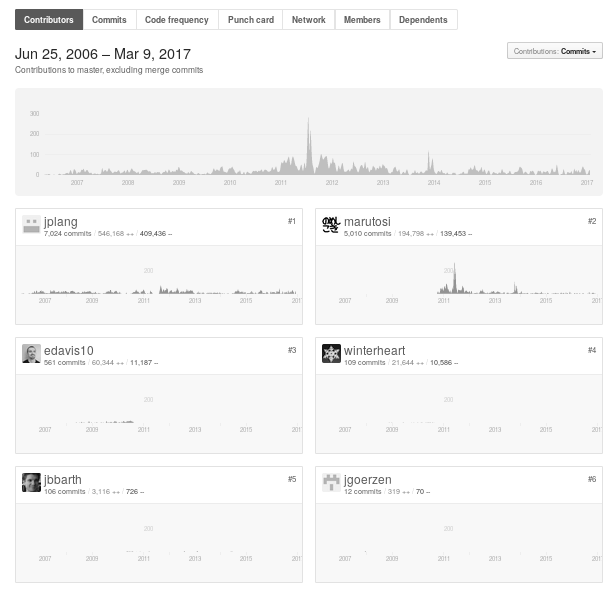
\includegraphics[width=0.8\linewidth]{./chapter-sugestoes-melhorias-fgrm/img/redmine_contribuidores.png}
	\caption{Lista de contribuidores do projeto Redmine}
\label{fig:redmine_contribuidores}
\end{figure}

\subsubsection{Desenho do Questionário}
\label{ssub:sug_melhoria_desenho_questionario}

A fim de coletar a opinião dos participantes foi utilizado um questionário
eletrônico produzido através da ferramenta \textit{Survey
	Gizmo}\footnote{\url{https://surveygizmo.com}}. O questionário foi desenhado
com a premissa de ser respondido em um prazo curto, de preferência entre 5 e 10
minutos. Neste sentido as perguntas foram organizadas em dois grupos principais.
As questões do primeiro grupo têm por objetivo coletar a opinião dos
profissionais sobre a relevância da recomendação proposta e o grau de
dificuldade de implementá-la. As perguntas foram estruturadas como uma escala
Likert em que o respondente deveria fornecer o seu nível de concordância para as
declarações que lhe são apresentadas. No segundo grupo as perguntas visam
estamos interessados na formação de base (background) dos profissionais. Optamos
por definir cada uma das questões como não obrigatórios por entendermos que a
impossibilidade ou o não interesse em responder uma determinada pergunta impeça
ao participante de enviar os dados de outras que foram respondidas. A
Figura~\ref{} exibe uma parte do formulário utilizado neste estudo.

\todobegin{Incluir figura com o formulário}

\subsubsection{Processo de Aplicação}
\label{ssub:processo_de_aplicação}

O questionário foi encaminhado à amostra de interesse através de correio
eletrônico. O endereço foi coletado diretamente do projeto hospedado no Github.
Foi desenvolvido um \textit{script} na linguagem Python que permitia coletar o
endereço de e-mail e automatizar o processo de envio. As mensagem foram
personalizadas de modo a identificar o nome do usuário e o projeto do Github
com base no template exibido a seguir.

\todobegin{Incluir o quadro com o template de envio das mensagens.}

O processo de envio consistia ainda de uma segunda mensagem de ``lembrete'' após
dois dias. Esta estratégia foi adotada com base em estudos que discutem
resultados em que o reenvio pode ser um dos fatores que aumentem a taxa de
participação em levantamentos por questionários realizados através da
web~\cite{fan2010factors}.

\section{Discussão}
\label{sec:sug_melhoria_discussao}

\section{Ameaças à Validade}
\label{sec:sug_melhoria_ameacas}

\section{Resumo do Capítulo}
\label{sec:sug_melhoria_resumo}
